\section{Analysis Procedure} \label{sec:ana}
% \begin{flushleft}
%    \subsection{Analysis overview}
The goal of TASEH is to find the axion signal hidden in the noise. In 
order to achieve this, the analysis procedure includes the following steps:
    \begin{enumerate}
        %\item Read raw data (I, Q) from tdms file and do Fast Fourier transform every 1 millisecond of spectrum, then average all over spectra in 1 second to get power spectrum.
        \item Perform fast Fourier transform (FFT) on the 
time-dependent spectrum to obtain the frequency-dependent spectrum.
        %\item Divide the measured power by the gains from the receiver chain to retrieve real power from cavity.
        %\item HEMT drift to predict noise and gain from the environmental parameters.
        %\item Use the results of high-electron-mobility-transistor(HEMT) drifting (see Section \ref{hemt_drifting}) to predict adding noise and gain; the input environmental parameters include monitoring temperatures, voltages of power supplies, etc.
        %\item Use Savitzky-Golay filter \cite{SGFilter} to remove the spectrum structure, then subtract the mean power.
        \item Apply the Savitzky-Golay (SG) filter to remove the 
Lorentzian structure of the frequency-dependent spectrum.
        \item Combine all power spectra from different frequency scans with 
the weighting algorithm.
        %\item Cause the expected Axion bandwidth, and our frequency resolution is 1KHz, so we need to merge the bin.
        \item Merge bins in the combined spectrum to maximize the SNR. 
%        %\item Set threshold at ${3.355\ \sigma}$.
       \item Rescan the frequency regions with candidates and set limits on 
      the axion-two-photon coupling \gagg\ if no candidates were found.
    \end{enumerate}

    The analysis was done by following the procedure similar to that 
adopted by the HAYSTAC experiment ~\cite{HAYSTACII}.
% \end{flushleft}

%\subsection{Tdms}
\subsection{Fast Fourier transform}
The in-phase $I(t)$ and quadrature $Q(t)$ components of the time-dependent 
data were recorded and saved in the TDMS 
(Technical Data Management Streaming) files - a 
binary format developed by National Instruments.
%Fast Fourier Transform (FFT) was performed to convert the data into frequency-dependent and into unit of power by using the equation:
The fast Fourier Transform (FFT) was performed to convert the data into 
frequency-dependent spectrum in which the measured power was calculated 
using the following equation:

\begin{equation}
\label{eq:4.1}
    \text{Power} = \frac{|\text{FFT}(I+i \cdot Q)|^{2}}{N \cdot 2R},
\end{equation}

where $N$ is the number of data points ($N  = 2000$ in the TASEH 
CD102 data), and $R$ is the resistance of the signal analyzer (50~$\Omega$).
The FFT was done for every one-millisecond subspectrum data. The integration 
time for each frequency scan was about 32-40 minutes, which resulted 
in 1920000 to 2400000 subspectra; an average over these subspectra gives 
the averaged frequency-dependent spectrum for each scan. 
The frequency resolution of each spectrum is 1~kHz. 

%\subsection{Gain}
%The net gain of our receiver chain includes: down conversion gain, Intermediate Frequency(IF)  attenuator, Radio Frequency(RF) attenuator and HEMT gain. The first three were the parameters set during data taking, the last one was estimated from calibration (Section \ref{sec:}). Fig.\ref{fig:Hemt_gain} shows the gain and noise from the HEMT calibration done before the data run.
%\newline
%After removing all the gains, we got the real power going out from the antenna of the cavity. The variation of the real power in time is shown in Fig. \ref{fig:over_temp}. One possible cause of this effect came from the additional gain variation that was not studied in the initial HEMT calibration before taking data. To investigate this issue, we did HEMT drifting to check the behavior of the gain over time.

%\begin{figure}[h]
%    \centering
%%    \includegraphics[width=0.4\textwidth,height = 0.25\textwidth]{Figure/CD099_HEMT.jpg}
%    \caption{ Gain and noise of HEMT before running data}
%    \label{fig:Hemt_gain}
%\end{figure}
%\begin{figure}[h]
%\centering
% %   \includegraphics[width=0.4\textwidth,height=4cm]{Figure/overall_temp.png}
%    \caption{Power over the time from step 1 to step 16}
%    \label{fig:over_temp}
%\end{figure}
%} // comment the paragraph of gain
%%\newpage


%\begin{figure}
%     \begin{subfigure}[b]{.24\textwidth}
%       \centering
%        \includegraphics[width=\linewidth,height=3cm]{Figure/before_sg.png}
%        \caption{Before SG filter}
%        \label{fig:before_sg}
%    \end{subfigure}%
%    \hfill
%    \begin{subfigure}[b]{.24\textwidth}
%        \centering
%        \includegraphics[width=\linewidth,height=3cm]{Figure/sg_result.png}
%        \caption{SG filter}
%        % \caption{Raw power of 1s data (blue line) and the output Savitzky-Golay filter (red line)}
%        \label{fig:sg_result}
%    \end{subfigure}%
%    \vskip\baselineskip
%    \begin{subfigure}[b]{.24\textwidth}
%        \centering
%        \includegraphics[width=\linewidth,height=3cm]{Figure/After_Sg.png}
%        \caption{After SG filter}
%        \label{fig:After_Sg}
%    \end{subfigure}%
%    \hfill
%    \begin{subfigure}[b]{.24\textwidth}
%        \centering
%        \includegraphics[width=\linewidth,height=3cm]{Figure/system_temp.png}
%        \caption{System temperature}
%        \label{fig:system_temp}
%    \end{subfigure}%
%    \caption{\textbf{(a)} The power spectra after average 12.5 hours of data. \textbf{(b)} Raw power of 1s data (blue line) and the output Savitzky-Golay filter (red line). \textbf{(c)} After dividing the sg filter's result in every step \textbf{(d)} The system temperature derived from $\mu$ and $\sigma$. }
    % \label{fig:fig}
%\end{figure}

% \begin{center}
% \begin{figure*}[!tbp]
% \centering
%     \begin{minipage}[t]{.24\textwidth}
%     \centering
%     \includegraphics[width=1\textwidth,
%     height = 0.75\textwidth]{Figure/before_sg.png}
%     \caption{Before SG filter}
%     \label{fig:before_sg}
%     \end{minipage}%
%     \hfill
%     \begin{minipage}[t]{.24\textwidth}
%     \centering
%     \includegraphics[width=1\textwidth,
%     height = 0.75\textwidth]{Figure/After_Sg.png}
%     \caption{After SG filter}
%     \label{fig:After_Sg}
%     \end{minipage}%
%     \hfill
%     \begin{minipage}[t]{.25\textwidth}
%     \centering
%     \includegraphics[width=1\textwidth,
%     height = 0.75\textwidth]{Figure/system_temp.png}
%     \caption{The system temperature calculate by $\mu$ and $\sigma$}
%     \label{fig:system_temp}
%     \end{minipage}%
% \end{figure*}
% \end{center}


%\subsection{Savitzky Golay filter}
\subsection{Remove the Lorentzian structure}
%Figure \ref{fig:sg_result} is the spectrum in each step, somehow they all have a similar structure, in order to remove this structure, we will use a Savitzky Golay filter in every second to smooth the data Figure \ref{fig:After_Sg}.

In the absence of the axion signal, the output data spectrum is simply the 
noise from the cavity and the amplification chain. If axions are present 
in the cavity, the signal will be buried in the noise because the 
signal power is very weak. Therefore, the Lorentzian structure of the raw 
output power spectrum, as shown in Fig.~\ref{fig:raw_sg_power}, is dominated 
by the noise of the system. 
Appendix~\ref{sec:cavitynoise} provides the derivation of the Lorentzian 
structure from the cavity noise due to a temperature difference 
between the DR environment and the cavity. The Savitzky Golay (SG) 
filter~\cite{SGFilter}, a digital filter that can smooth data without 
distorting the signal tendency, was applied to remove the structure of the  
background. The SG filter was performed on the averaged spectrum of each 
frequency scan by fitting adjacent points of successive sub-sets of data with 
an $n^\text{th}$-order polynomial. The result depends on two parameters: 
the number of 
data points used for fitting, the so-called window width, and the order of 
the polynomial. If the window is too wide, the filter will not remove small 
structures, and if it is too narrow, it may kill the signal. 
The window and the order were first chosen during the data taking based on 
the structure of data and the ratio of the raw data to the filter output. 
After the data taking, they were optimized by injecting an axion signal on top of 
the noise data and found that they were consistent with the original choice 
(see Section~\ref{sec:sys}). 

The raw averaged spectrum was divided by the output of the SG filter, then  
unity is subtracted from the ratio to get the normalized spectrum 
(Fig.~\ref{fig:raw_sg_power}).
Therefore, if the axion signal exists, a power excess will be above zero.
%After filtering, the normalized spectrum (Fig. \cite{fig:}) was obtained by dividing the raw spectrum by the output of the SG filter subtract 1. Therefore, if the signal exists, the excess power will be above 0.
During the data taking, the resonant frequency of the cavity was  
adjusted by the tuning bar so to scan a large range of frequencies and to 
reduce the uncertainty of the noise at the overlapped region. Therefore, the 
spectra of all the scans need to be combined to create one big spectrum. 
Before doing this, 
the normalized spectrum from each scan was rescaled by the system noise 
(detailed in Sec~\ref{sec:intronoise} and Sec~\ref{sec:calibration}) and the 
signal power with the Lorentzian cavity response taken into account. The 
rescaled spectrum, shown in 
Fig.~\ref{fig:raw_sg_power}, was computed with the following formula:

\begin{equation}
  \label{eq:respower_eqn}
  \delta_{ij}^\text{res} = \frac{k_{B}\tsys \Delta\nu }{P_{ij}^{s} h}\delta_{ij}^\text{norm},
\end{equation}

and the standard deviation of each bin is:
\begin{equation}
  \label{eq:ressigma_eqn}
  \sigma_{ij}^\text{res} = \frac{k_{B}\tsys\Delta\nu }{P_{ij}^{s} h}\sigma_{i}^\text{norm},
\end{equation}

where $\delta_{ij}^\text{norm}$ ($\delta_{ij}^\text{res}$) and 
$\sigma_{i}^\text{norm}$ ($\sigma_{ij}^\text{res}$) are the power and the 
standard deviation of the $j^\text{th}$ frequency bin from the 
normalized (rescaled) spectrum of the $i^\text{th}$ frequency scan. 
The $\Delta\nu$ is the bin 
width of spectrum (1~kHz) and  $P_{ij}^{s}$ is the KSVZ axion signal power. 
The $h = \frac{1}{1 + [2(\nu_{ij} - \nu_{ci})/\Delta\nu_{i}]^2}$ 
describes the Lorentzian response of the cavity, where 
$\Delta\nu_{i}$ is the cavity line width, which depends on the resonant 
frequency $\nu_{ci}$ and the loaded quality factor. 
%
If a signal appears in a certain frequency bin $j$, its expected power 
will vary depending on the bin position due to the cavity's 
Lorentzian response. The rescaling will take into account this effect.

\begin{figure} [htbp]
  \centering
  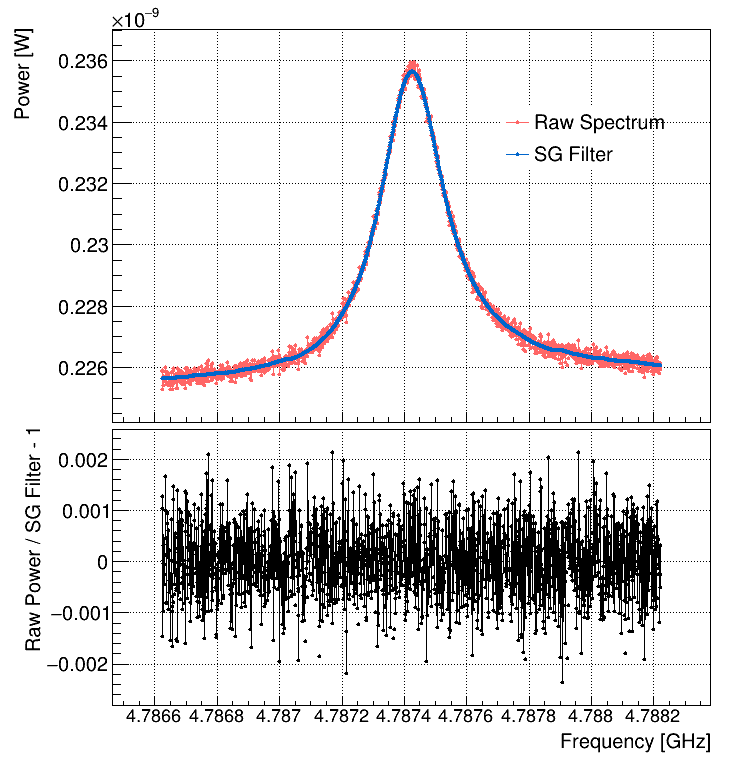
\includegraphics[width=0.38\textwidth,height = 0.4\textwidth]{figures/RawPower_SGPower_Ratio_vs_Freq_Step_0100.png}
  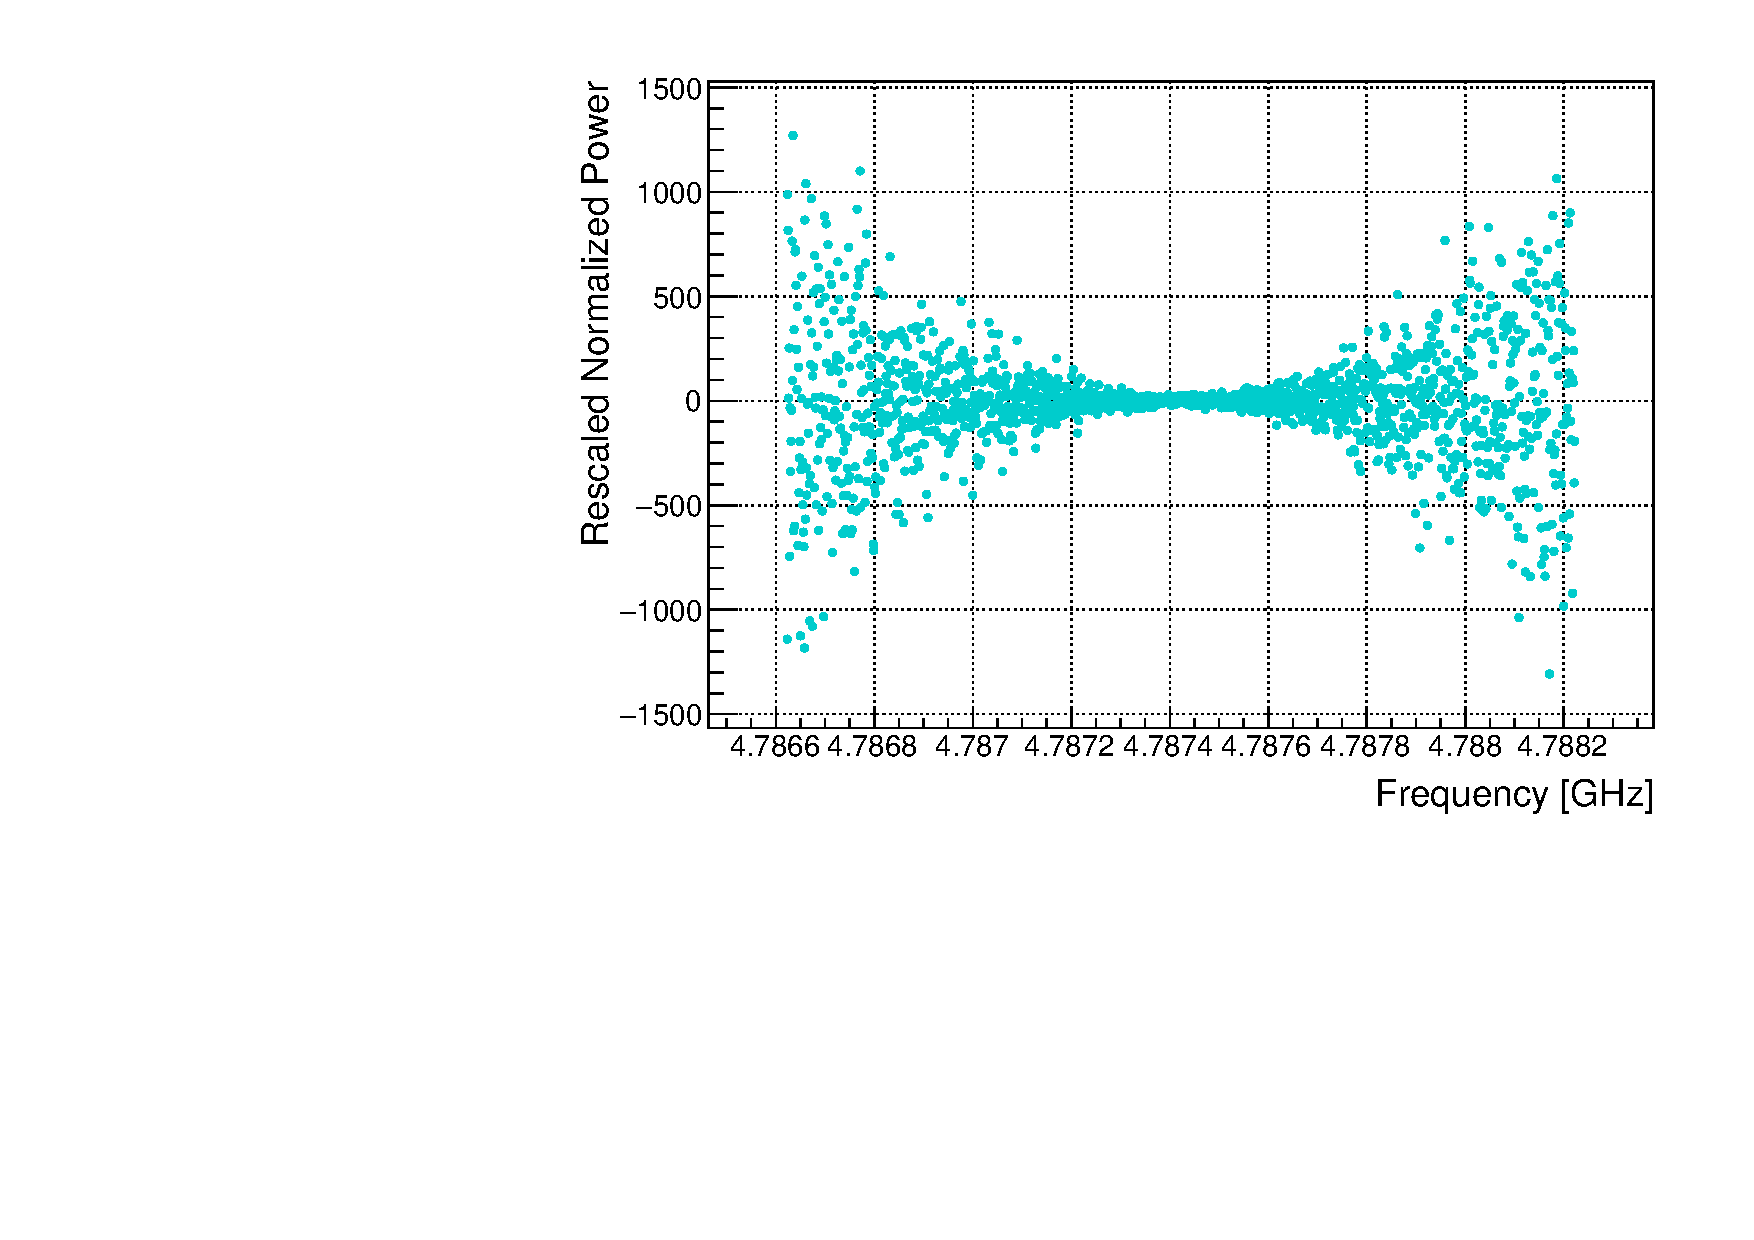
\includegraphics[width=0.52\textwidth,height = 0.4\textwidth]{figures/RescaledPower_vs_Freq_Step_0100.pdf}
  \caption{Left: Upper panel: The raw power spectrum (blue) and the output of 
the SG filter (red) of one scan. Bottom panel: The normalized spectrum,  
derived by taking the ratio of the raw spectrum to the SG filter and 
subtracting unity from the ratio. 
  Right: The rescaled power spectrum, obtained by multiplying the normalized 
power with the ratio of the system noise to the expected axion signal power, 
with the Lorentzian response of the cavity taken into account.}
  \label{fig:raw_sg_power}
\end{figure}

%\begin{figure} [htbp]
%  \centering
%  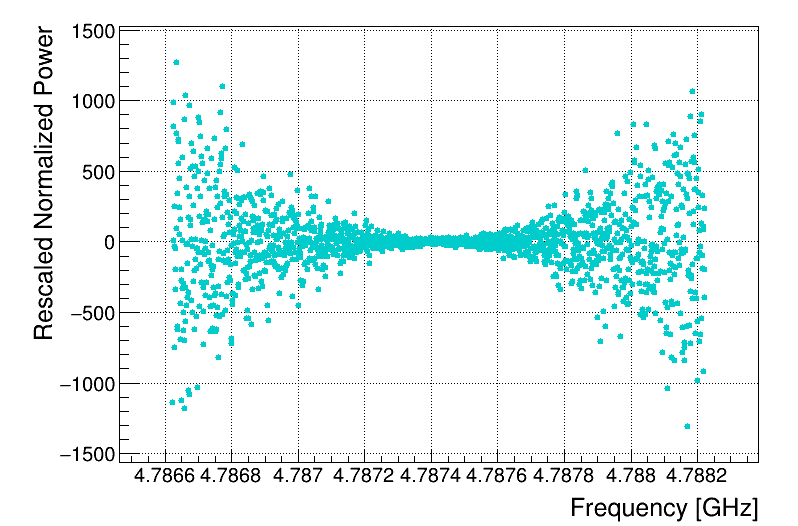
\includegraphics[width=0.4\textwidth,height = 0.4\textwidth]{figures/RescaledPower_vs_Freq_Step_0100.png}
%  \caption{Rescaled power spectrum obtained by multiplying the normalized power with system noise and dividing expected axion signal power% taking the Lorentzian shape of cavity into account}
%  \label{fig:res_spectrum}
%\end{figure}



%First we will choose a window and a order, then move the window and fit the data a with a polynomial with chosen order, it is a kind of generalization  moving average characterized, if the windows is too big, then it will not remove small structures, if it too small, it may kill the signal, you can see that choosing an appropriate window is important, a way to test if the windows are appropriate is to see the system temperature calculated by  $\mu$ and $\sigma$.

%\begin{equation}
%    \label{eq:ts_mu}
%    \mu = k_{B} \cdot T_{S} \cdot \Delta \nu 
%\end{equation}
%\begin{equation}
%    \label{eq:ts_sigma}
%    \sigma = \frac{k_{B} \cdot T_{S} \cdot \Delta \nu}{\sqrt{N}}
%\end{equation}

%If we treat the spectrum after the SG filter as a pure noise, we know that the system temperature of a white noise can be calculated by $\mu$ and $\sigma$ (Eq.\eqref{eq:ts_mu}) (Eq.\eqref{eq:ts_sigma}),
%where $k_{B}$ is the Boltzmann constant, $T_{S}$ is the system temperature, $\Delta \nu$ is the frequency resolution and N is the number of averaging. \\
%If the chosen window is appropriate, the system temperature estimated from $\mu$ and $\sigma$ should be consistent  with each other. \\

%We also did some studies to check if the SG filter removed the axion signal. Assuming a signal bandwidth of 5 kHz, we added the signal into noise spectrum and applied the SG filter. The result shows that the filter does not suppress the axion signal as given in Fig.\ref{fig:weighted_snr}.

%about whether the sg filter will remove the Axion signal, assuming the Axion signal bandwidth is 5KHz, add the signal in a white noise and apply the sg filter , the results show that it will not affect much before and after use, after divide the sg filter result, we will subtract 1 to make the value become 1.

%\begin{figure}[h]
%    \begin{minipage}[h]{.5\textwidth}
%    \centering
%    \includegraphics[width=0.8\textwidth, height = 0.5\textwidth]{Figure/sg_simulation.png}
%    \caption{The simulation for testing the effect of SG filter.}
%    \label{fig:weighted_snr}
%%    \end{minipage}%
%\end{figure}
%\begin{figure}[h]
%    \begin{minipage}[t]{.5\textwidth}
%    \centering
%    \includegraphics[width=0.8\textwidth,height = 0.5\textwidth]{Figure/weighted_snr.png}
%    \caption{Weighed SNR}
%    \label{fig:weighted_snr}
%%    \end{minipage}%
%\end{figure}

\subsection{Combine the spectra with the weighting algorithm} 
\label{sec:weighting_algorithm}

The purpose of the weighting algorithm is to add different spectra vertically,
 particularly for the frequency bins that appear in multiple spectra.  
Each spectrum was collected with a different cavity resonant frequency. 
Therefore, if a signal appears in a certain frequency bin $j$, due to the
 difference in resonant frequency and Lorentzian response, the expected signal
 power will be different in each spectrum $i$. The weighting algorithm is 
expected to take this into account with a weight calculated for each bin $j$ of
 the normalized and rescaled spectrum $i$, as defined in Eq.~\eqref{eq:weight}.
The weighted power $\delta^\text{com}_{n}$ and the standard deviation 
$\sigma^\text{com}_{n}$ of the $n^\text{th}$ bin in the combined spectrum are 
calculated using Eq.~\eqref{eq:comb_power} and Eq.~\eqref{eq:comb_sigma}, 
respectively. The SNR$^\text{com}_{n}$ is the ratio of 
$\delta^\text{com}_{n}$ to 
$\sigma^\text{com}_{n}$ as given in Eq.~\eqref{eq:comb_snr}. 
Figure~\ref{fig:power_sigma_comb} and Fig.~\ref{fig:SNR_comb} show the power, 
the standard deviation, and the SNR of the combined spectrum, respectively.


\begin{equation}
    \label{eq:weight}
    %    {w_{n}}^{i} = \frac{h \cdot p}{(\sigma_{n}^{i})^{2}}
    {w_{ij}} = \frac{1}{(\sigma_{ij}^\text{res})^{2}},
\end{equation}

\begin{equation}
    \label{eq:comb_power}
    \delta_{n}^\text{com} = \frac{ \sum_{1}^{k}\delta_{ij}^\text{res} \cdot {w_{ij}}}{\sum_{1}^{k} {w_{ij}}},
\end{equation}
\begin{equation}
    \label{eq:comb_sigma}
    \sigma_{n}^\text{com} = \frac{ \sqrt{\sum_{1}^{k}(\sigma_{ij}^\text{res} \cdot {w_{ij}})^2}}{\sum_{1}^{k} {w_{ij}}},
\end{equation}
\begin{equation}
    \label{eq:comb_snr}
    \text{SNR}_{n}^\text{com} = \frac{\delta^\text{com}_{n}}{\sigma^\text{com}_{n}}= \frac{\sum_{1}^{k}\delta_{ij}^{res} \cdot {w_{ij}}}{ \sqrt{\sum_{1}^{k}(\sigma_{ij}^{res} \cdot {w_{ij}})^2}},
\end{equation}

with $i$ running from 1 to $k$ where $k$ is the 
number of spectra that share the same frequency bin $j$.

\begin{figure}[h]
    \centering
    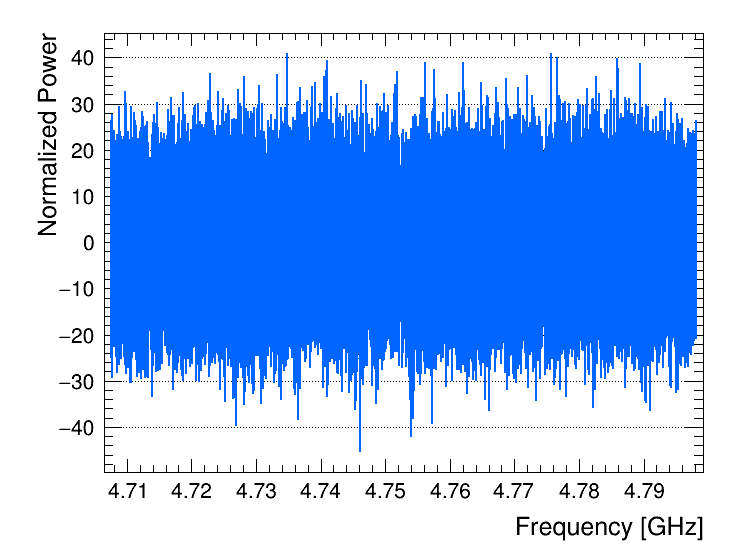
\includegraphics[width=0.4\textwidth,height = 0.3\textwidth]{figures/Power_CombSpectrum_AxionRun_AllSteps_Rescan_SG4_W201_LqWeight.png}
    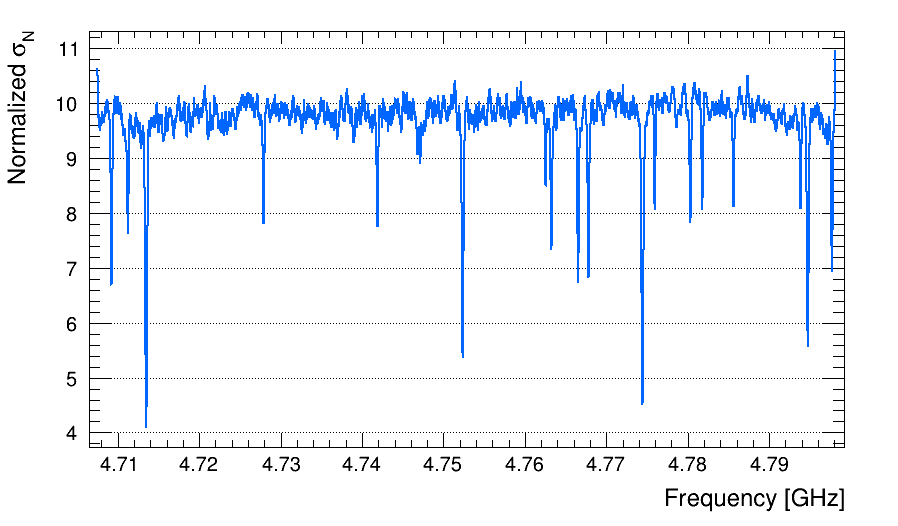
\includegraphics[width=0.4\textwidth,height = 0.3\textwidth]{figures/Sigma_CombSpectrum_AxionRun_AllSteps_Rescan_SG4_W201_LqWeight.png}
    \caption{The combined power $\delta$ following Eq.~\eqref{eq:comb_power} 
(left) and the standard deviation $\sigma$ derived from 
Eq.~\eqref{eq:comb_sigma} (right).}
    \label{fig:power_sigma_comb}
\end{figure}

\begin{figure}[hbt!]
    \centering
    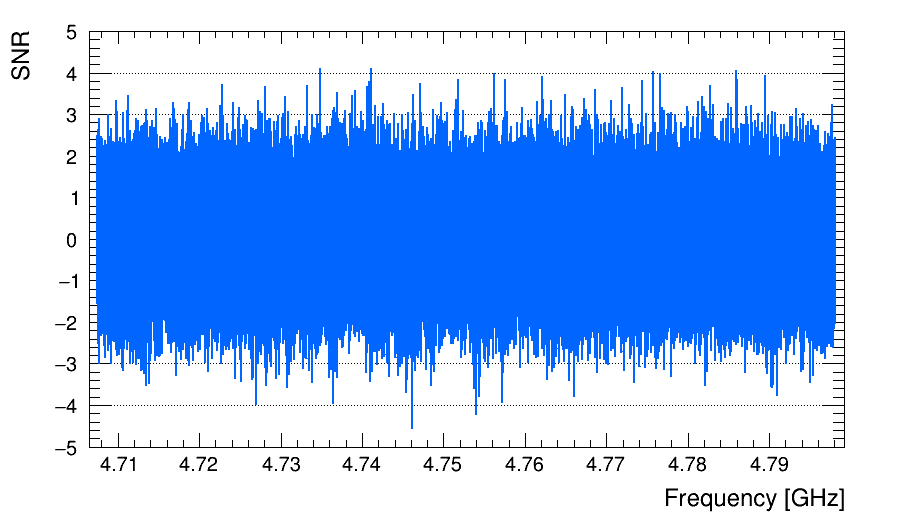
\includegraphics[width=8.6cm]{figures/SNR_CombSpectrum_AxionRun_AllSteps_Rescan_SG4_W201_LqWeight.png}
    \caption{The signal-to-noise ratio (SNR) calculated using 
Eq.\eqref{eq:comb_snr} of the combined spectrum. }
    \label{fig:SNR_comb}
\end{figure}


%where ${\delta_n^i}$ and ${\sigma_n^i}$ are the measured power and the corresponding standard deviation of the ${n^{\mathrm{th}}}$ frequency bin of the ${i^{\mathrm{th}}}$ spectrum., From the weighted power in ${n^{th}}$ bin in Eq.\eqref{eq:weighted_power}, and weighted $\sigma$ in Eq.\eqref{eq:weighted_sigma}, we can get our Signal to noise ratio as Eq.\eqref{eq:weighted_SNR}

\subsection{Merge bins}
\label{sec:merge}

The expected axion bandwidth is about 5~kHz at the frequency of 5~GHz. In 
this paper, the interested frequency range is \flo -- \fhi~GHz and the bin 
width is 1~kHz. Therefore, in order to maximize the SNR, five consecutive 
bins with overlapping of the combined spectrum were merged to construct a 
final spectrum.
The purpose of overlapping is to avoid the signal power broken into different 
neighboring bins of the merged spectrum. Before defining the weights for 
merging, 
the power and the standard deviation of each bin in the combined spectrum are 
multiplied with $M=5$: $\delta^{c}_n \rightarrow M\delta^\text{com}_n$ and 
$\sigma^{c}_n \rightarrow M \sigma^\text{com}_n$. This rescaling gives the 
expected mean of the normalized power $\mu^\text{com}_k = 1$ if a KSVZ axion 
signal power leaves a fraction 1/$M$ of its power in the $k^\text{th}$ 
bin of the combined spectrum.
Then the maximum likelihood weights, defined in Eq.~\eqref{eq:merge_weight} based on the Maxwellian line shape for axions [Eq.~\eqref{eq:simplesignal}], 
were used to build the merged spectrum. 



\begin{equation}
    \label{eq:merge_weight}
    w_{n} = \frac{L_{n}}{(\sigma_{n}^{c})^{2}} = \frac{L_{n}}{(M\sigma_{n}^\text{com})^{2}},
\end{equation}

where $M = 5$ is the number of merged bins.

%\begin{equation}
%    \label{eq:axion_line_shape}
%    f(\nu) = \frac{2}{\sqrt{\pi}}\sqrt{\nu - \nu_a} \left( \frac{3}{\nu_a \big \langle \beta^{2} \big \rangle }\right)^{\frac{3}{2}} e^{- \frac{3(\nu-\nu_a)}{\nu_a \big \langle \beta^{2} \big \rangle}}
%\end{equation}

\begin{equation}
    \label{eq:Lq_integtal}
    L_{n} = M \int_{\nu_a +\delta\nu_m + n\Delta\nu}^{\nu_a +\delta\nu_m + (n+1)\Delta\nu} f(\nu) \,d\nu,
\end{equation}


where $n = 1,..,M$, $\nu_a$ is the axion frequency, $\delta\nu_m$ is the misalignment between $\nu_a$ and the lower bin boundaries
in the combined spectrum and $\Delta\nu =$ 1 kHz is the bandwidth.

%where $L_q$ is the integral of the line shape from the lower edge to higher 
%edge of ${q^{th}}$ bin. 
The power, the standard deviation and the SNR of the merged spectrum are:

%We have a weight Eq.\eqref{eq:merge_weight}, where Lq is the area in ${q^{th}}$ bin and $\sigma_{q}$ is the weighted $\sigma$ in the $q^{\mathrm{th}}$ bin , Eq.\eqref{eq:axion_line_shape} is the axion CDM(cold dark matter) line shape, where $\big \langle \beta^{2} \big \rangle = \big \langle v^{2} \big \rangle /c^{2}$ and $\big \langle v^{2} \big \rangle = (270km/s)^{2}\ , \big \langle v^{2} \big \rangle$ is the squared virial velocity. Eq.\eqref{eq:L_q_integtal},

\begin{equation}
    \label{eq:merged_power}
    \delta_{g}^\text{merged} = \frac{ \sum_{n = 1}^{M}\delta_{g+n-1}^{c} \cdot {w_{n}}}{\sum_{n = 1}^{M} {w_{n}}}
\end{equation}

\begin{equation}
    \label{eq:merged_sigma}
    \sigma_{g}^\text{merged} =  \frac{ \sqrt{\sum_{n = 1}^{M} (\sigma_{n}^{c})^2 \cdot {w_{n}^2}}}{\sum_{n = 1}^{M} {w_{n}}}
\end{equation}

\begin{equation}
    \label{eq:merged_snr}
    \text{SNR}_{g}^\text{merged} = \frac{\delta^\text{merged}_{g}}{\sigma^\text{merged}_{g}} = \frac{\sum_{n = 1}^{M}\delta_{n}^{c} \cdot {w_{n}}}{ \sqrt{\sum_{n = 1}^{M} (\sigma_{n}^{c})^2 \cdot {w_{n}^2}}}
\end{equation}

where $g = 1,..,N-M+1$ is the number of bins in the final spectrum.


%Adding adjacent bin with a weight Eq.\eqref{eq:merged_power} Eq.\eqref{eq:merged_sigma}, where k is the number of adjacent bin to be merged, q is ${q^{th}}$ merged bin, with Eq.\eqref{eq:merged_sigma}, we can get our weighted merged power spectrum FIG.\ref{fig:merged_data}.


\subsection{Rescan and set limits on \gagg} 
Before the collection of the CD102 data, a 5$\sigma$ SNR target was chosen, 
which corresponds to a candidate threshold of 3.355$\sigma$ at 95\% confidence.
 After the merging as described in Section~\ref{sec:merge}, if there were 
any potential signal with an SNR larger than 
3.355$\sigma$, a rescan would be proceeded to check if it were a real signal or 
a statistical fluctuation. 
The procedure of the CD102 data taking was to perform a rescan after 
covering every 10~MHz; the rescan was done by adjusting the tuning rod of the 
cavity so to match the resonant frequency to the frequency of the candidate. 
Most of the candidates were from the fluctuations because they were gone 
after a few rescans. 
Some of them reached SNR > 4$\sigma$ after rescanning; a portable 
antenna outside the DR was used to probe if they came from external sources. 
During the data taking, external signals at two frequencis from the instruments
in the laboratory were detected. More details can be found in the 
TASEH instrumentation paper~\cite{TASEHInstrumentation}. 
Figure~\ref{fig:power_sigma_merged} and Fig.~\ref{fig:SNR_merged} show the 
power, the standard deviation, and the SNR of the merged spectrum after 
performing the rescan, respectively. 

Since no candidates were found after the rescan, an upper limit on 
the signal power $P_s$ was derived by setting $P_s$ equal to 
$5\sigma_{q}^\text{merged}$ for a certain frequency bin $q$ in the merged 
spectrum.  Then, the 95\% C.L. limits on the dimensionless parameter 
\ggamma\ and the axion-two-photon coupling \gagg\ could be derived 
according to Eq.~\eqref{eq:ps} and Eq.~\eqref{eq:grelation}. 
See Section~\ref{sec:results} for the final limits including the systematic 
uncertainties.

\begin{figure}[h]
    \centering
    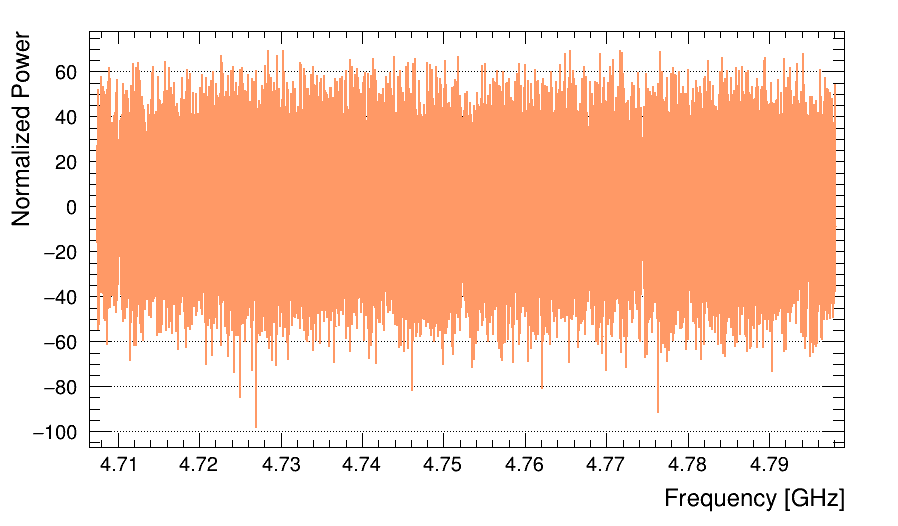
\includegraphics[width=0.4\textwidth,height = 0.3\textwidth]{figures/Power_GrandSpectrum_AxionRun_AllSteps_Rescan_Merged_5bin_SG4_W201_LqWeight.png}
    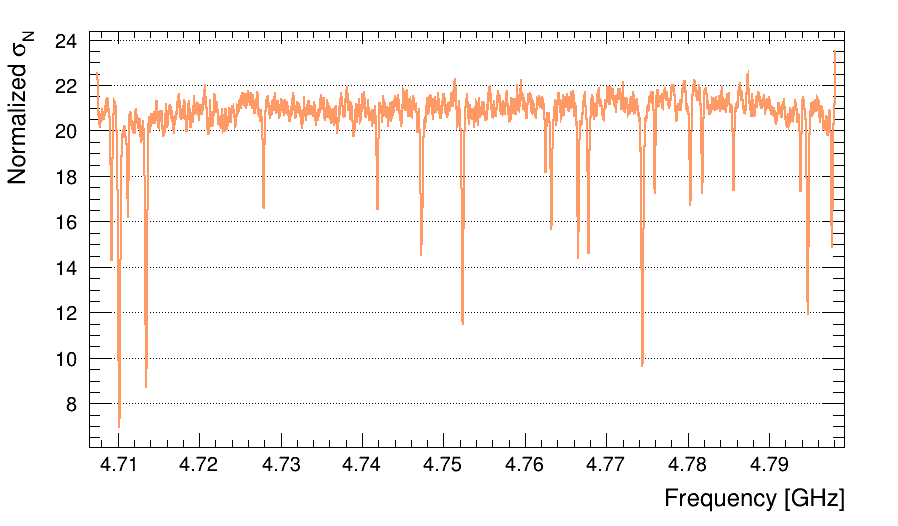
\includegraphics[width=0.4\textwidth,height = 0.3\textwidth]{figures/Sigma_GrandSpectrum_AxionRun_AllSteps_Rescan_Merged_5bin_SG4_W201_LqWeight.png}
    \caption{The merged power $\delta$ following Eq.~\eqref{eq:merged_power} 
(left) and the standard deviation $\sigma$ derived from Eq.~\eqref{eq:merged_sigma} (right).}
    \label{fig:power_sigma_merged}
\end{figure}

\begin{figure}[hbt!]
    \centering
    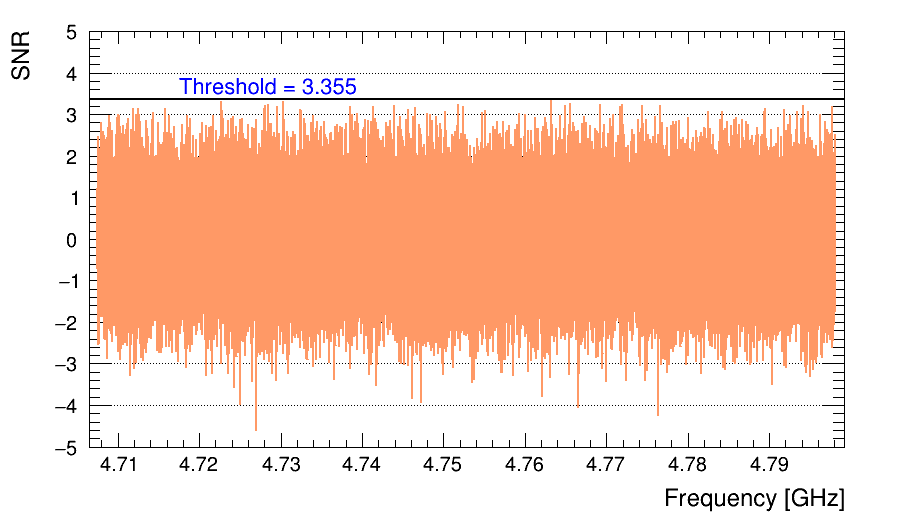
\includegraphics[width=8.6cm]{figures/SNR_GrandSpectrum_AxionRun_AllSteps_Rescan_Merged_5bin_SG4_W201_LqWeight.png}
    \caption{The signal-to-noise ratio (SNR) calculated using Eq.~\eqref{eq:merged_snr} for the merged spectrum after rescan. 
No candidate exceed the threshold of 
$3.355\sigma$ (solid-black horizontal line). }
    \label{fig:SNR_merged}
\end{figure}
